\documentclass[letterpaper]{article}

\usepackage[margin=1in]{geometry}
\usepackage{graphicx}
\usepackage{cleveref}


\title{Trundl: An Exploration of Particle Filters}
\author{Jeremy Silver}
\date{\today}
\begin{document}
\maketitle

\abstract{}



\section{Definition}

\subsection{Project Overview}

For this project, I decided to look at the problem of robot localization and pathfinding under uncertainty. I first started to understand how interesting a problem this could be when I saw a video from Sebastian Thrun's AI for Robotics course at Udacity. The video showed a particle filter 


\begin{figure}\label{fig:localization-example}
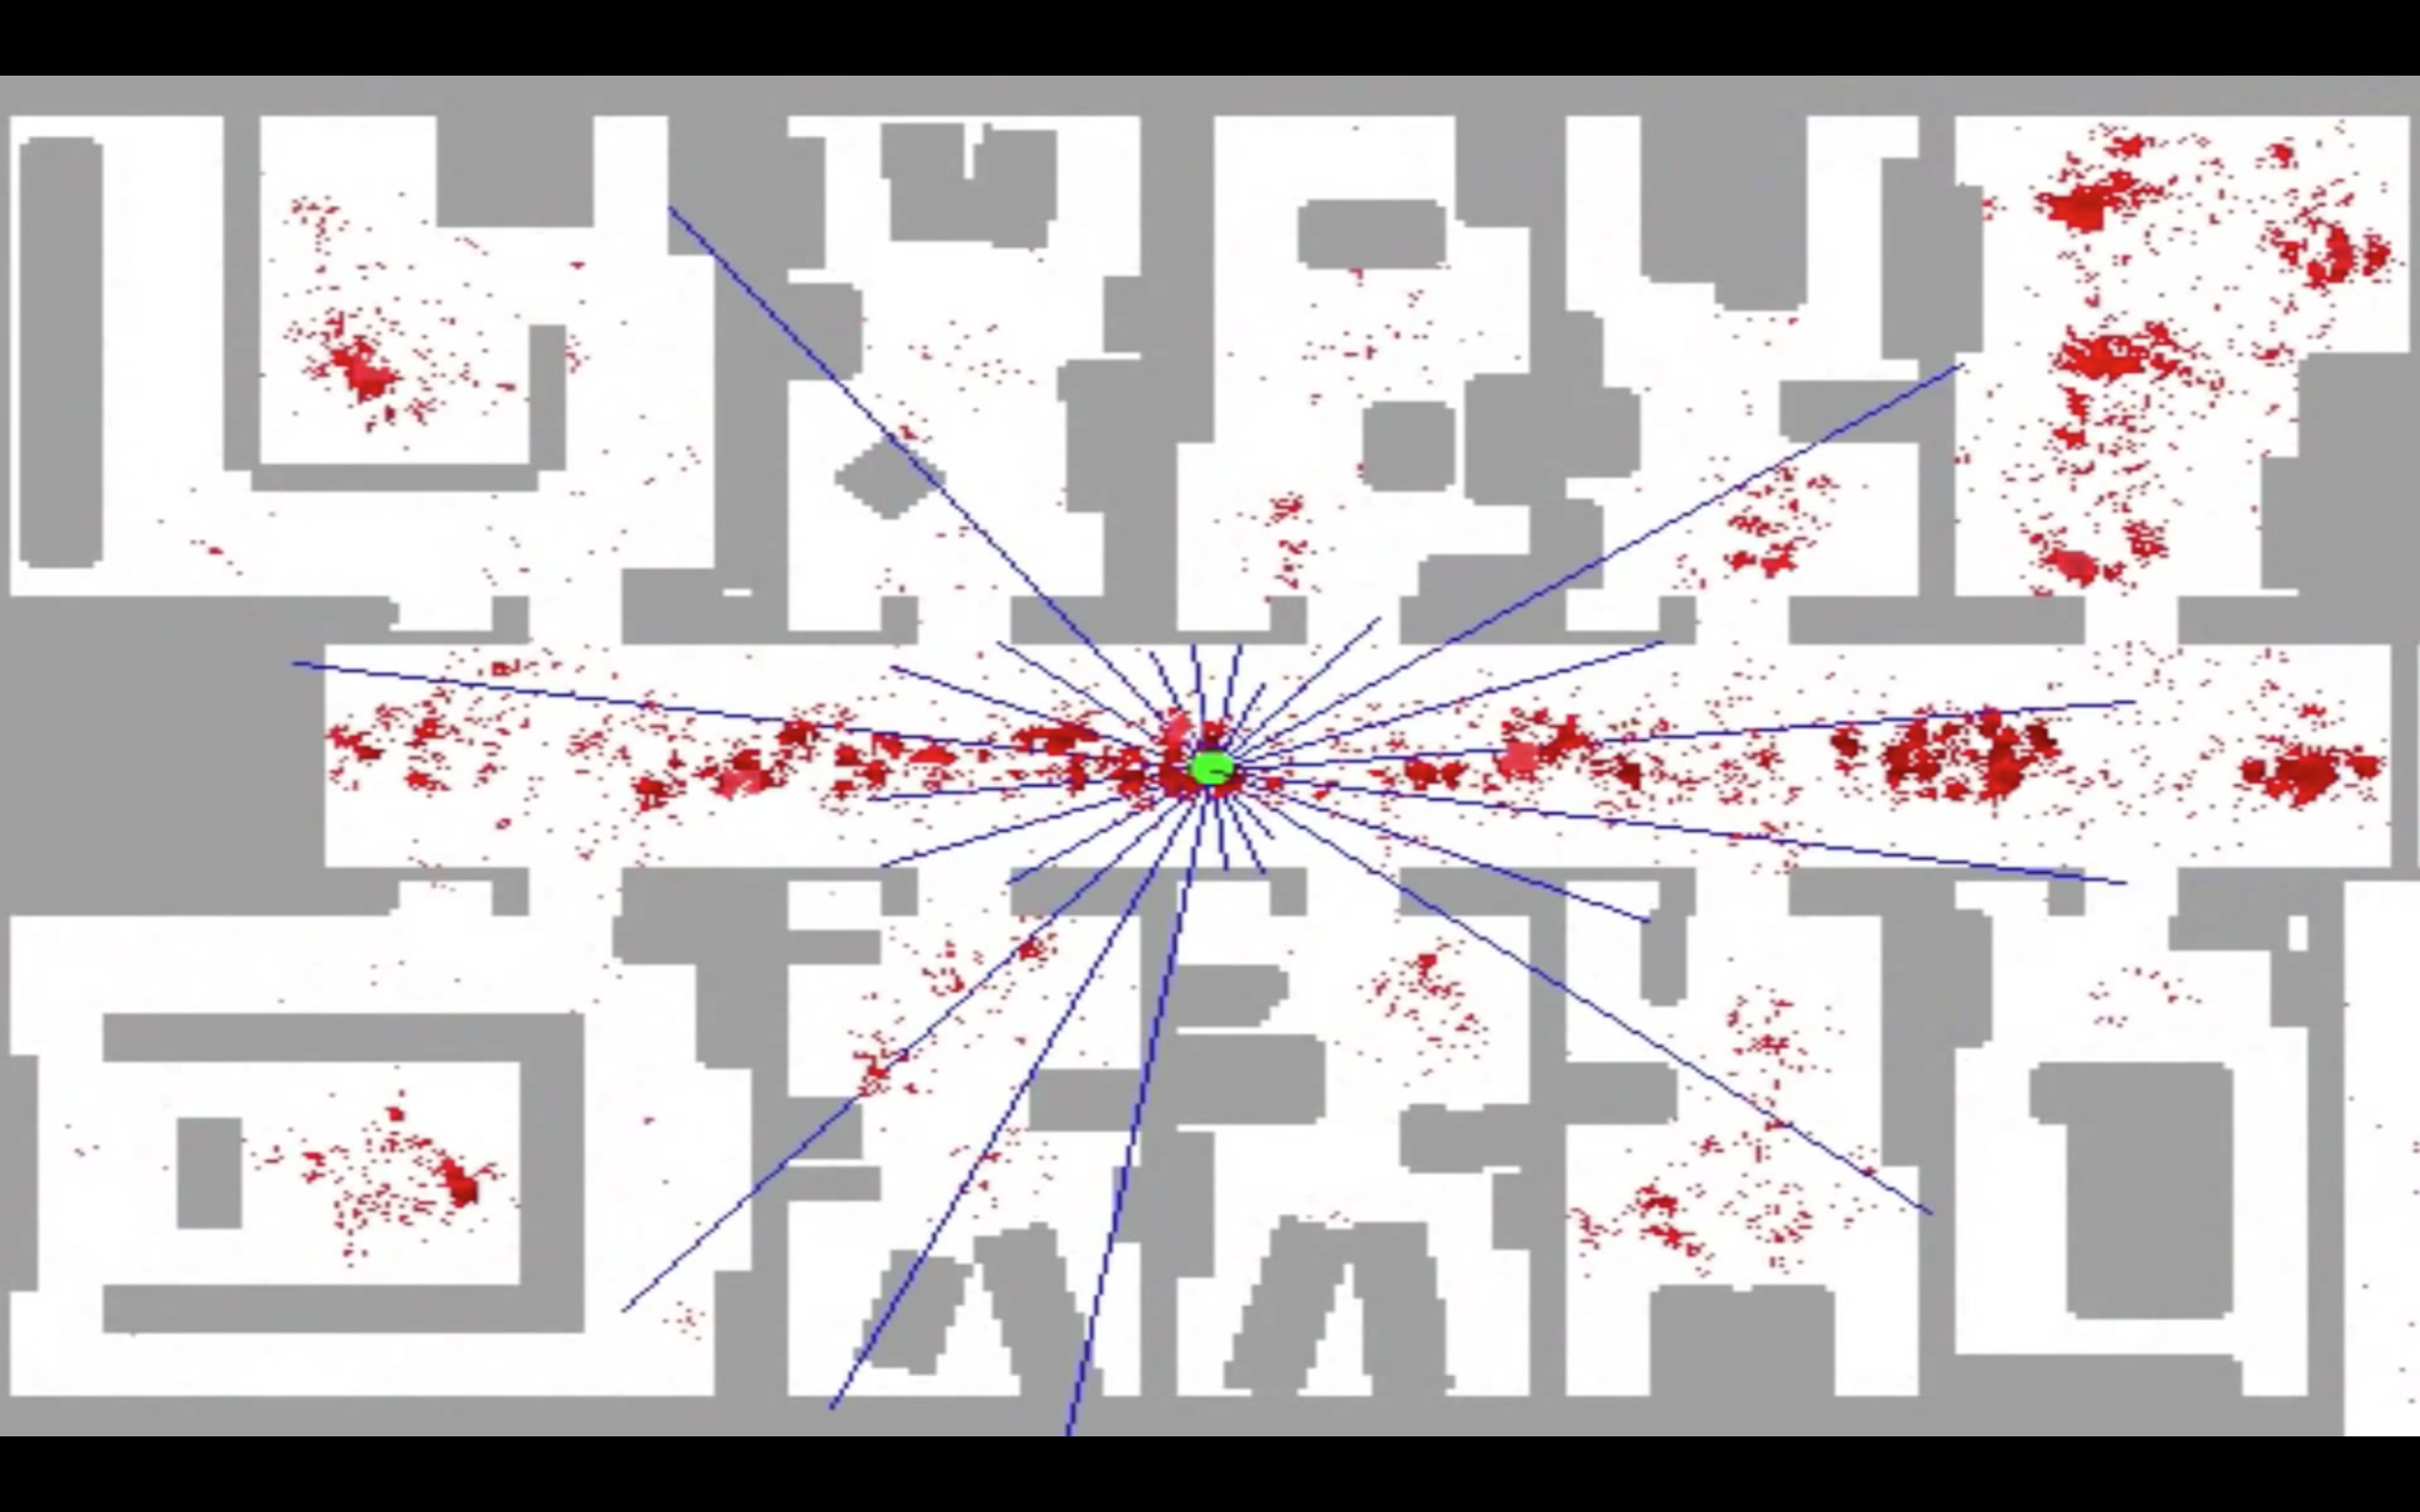
\includegraphics[width=.5\linewidth]{images/localization-example.png}



\end{figure}







\bibliography{my_bib}{}
\bibliographystyle{plain}

\end{document}
